%%% File: ./inputs/parts/HIPPOCAMPAL_COMPLEX.tex

%%% %%%%%%%%%%%%%%%%%%%%%%%%%%%%%% BEGIN HIPPOCAMPAL COMPLEX %%%%%%%%%%%%%%%%%%%%%%%

Figure~{\urlh{#fig_Hippocampus_Anatomy_and_Physiology}{\ref{fig_hippo}}} provides a glimpse of how we construct memories of our experience and subsequently retrieve those memories to support a diverse range of cognitive strategies. In this case, the {\it{hippocampus}} will play a central role as did the basal ganglia in the previous example. In the next section, we explore how the basal ganglia work in concert with the hippocampus to support reinforcement learning. For now, our goal is simply to describe the process whereby we consolidate and then encode experience. In doing so we take the opportunity to talk about the process whereby we retrieve memories, reconstruct a version of that past experience to perform counterfactual inference and imagine possibilities that we have never actually experienced. 

%%% %%%%%%%%%%%%%%%%%%%%%%%%%%%%%%%%%%%%%%%%%%%%%%%%%%%%%%%%%%%%%%%%%%%%%%%%%%%%

%%% Figure~{\urlh{#fig_Hippocampus_Anatomy_and_Physiology}{\ref{fig_hippo}}}
\begin{figure}
%
  \begin{center}
%    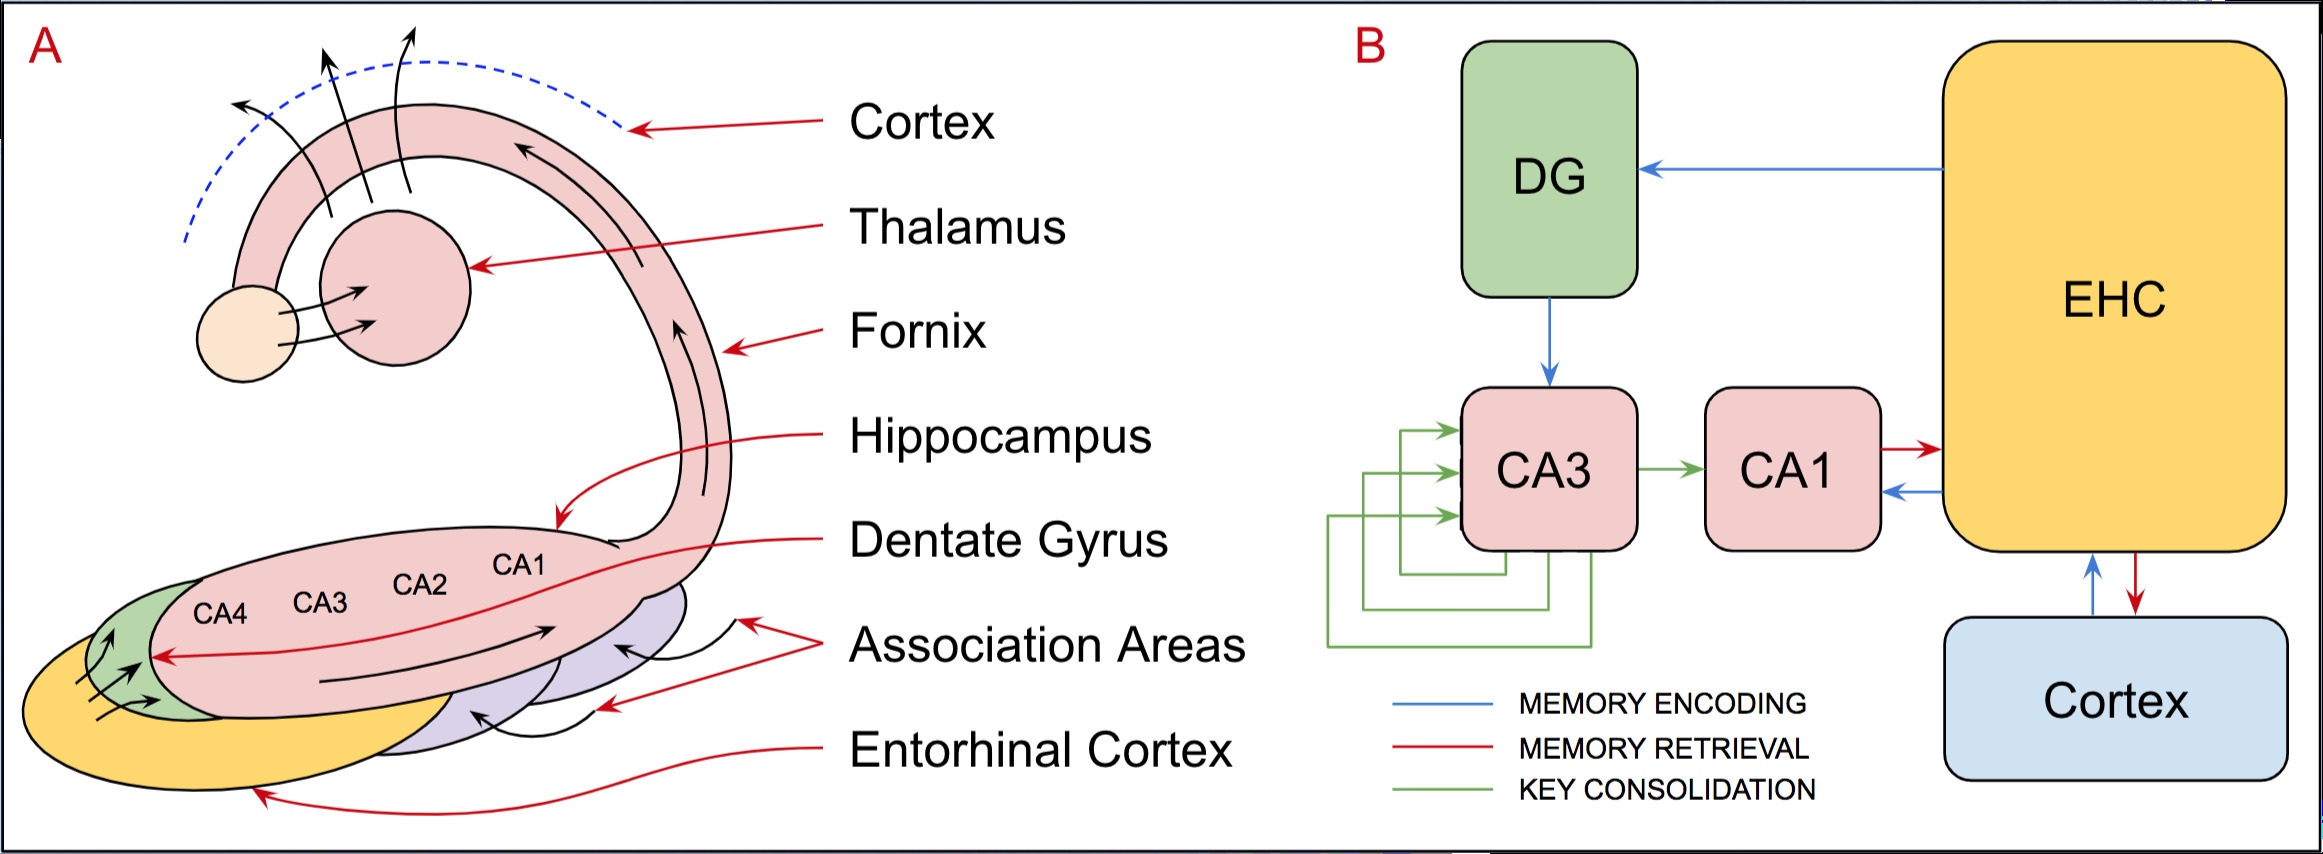
\includegraphics[width=10.0in]{./figures/Hippocampus_Anatomy_and_Physiology.png} %%% 2362 × 900 pixels @ 72 per inch
    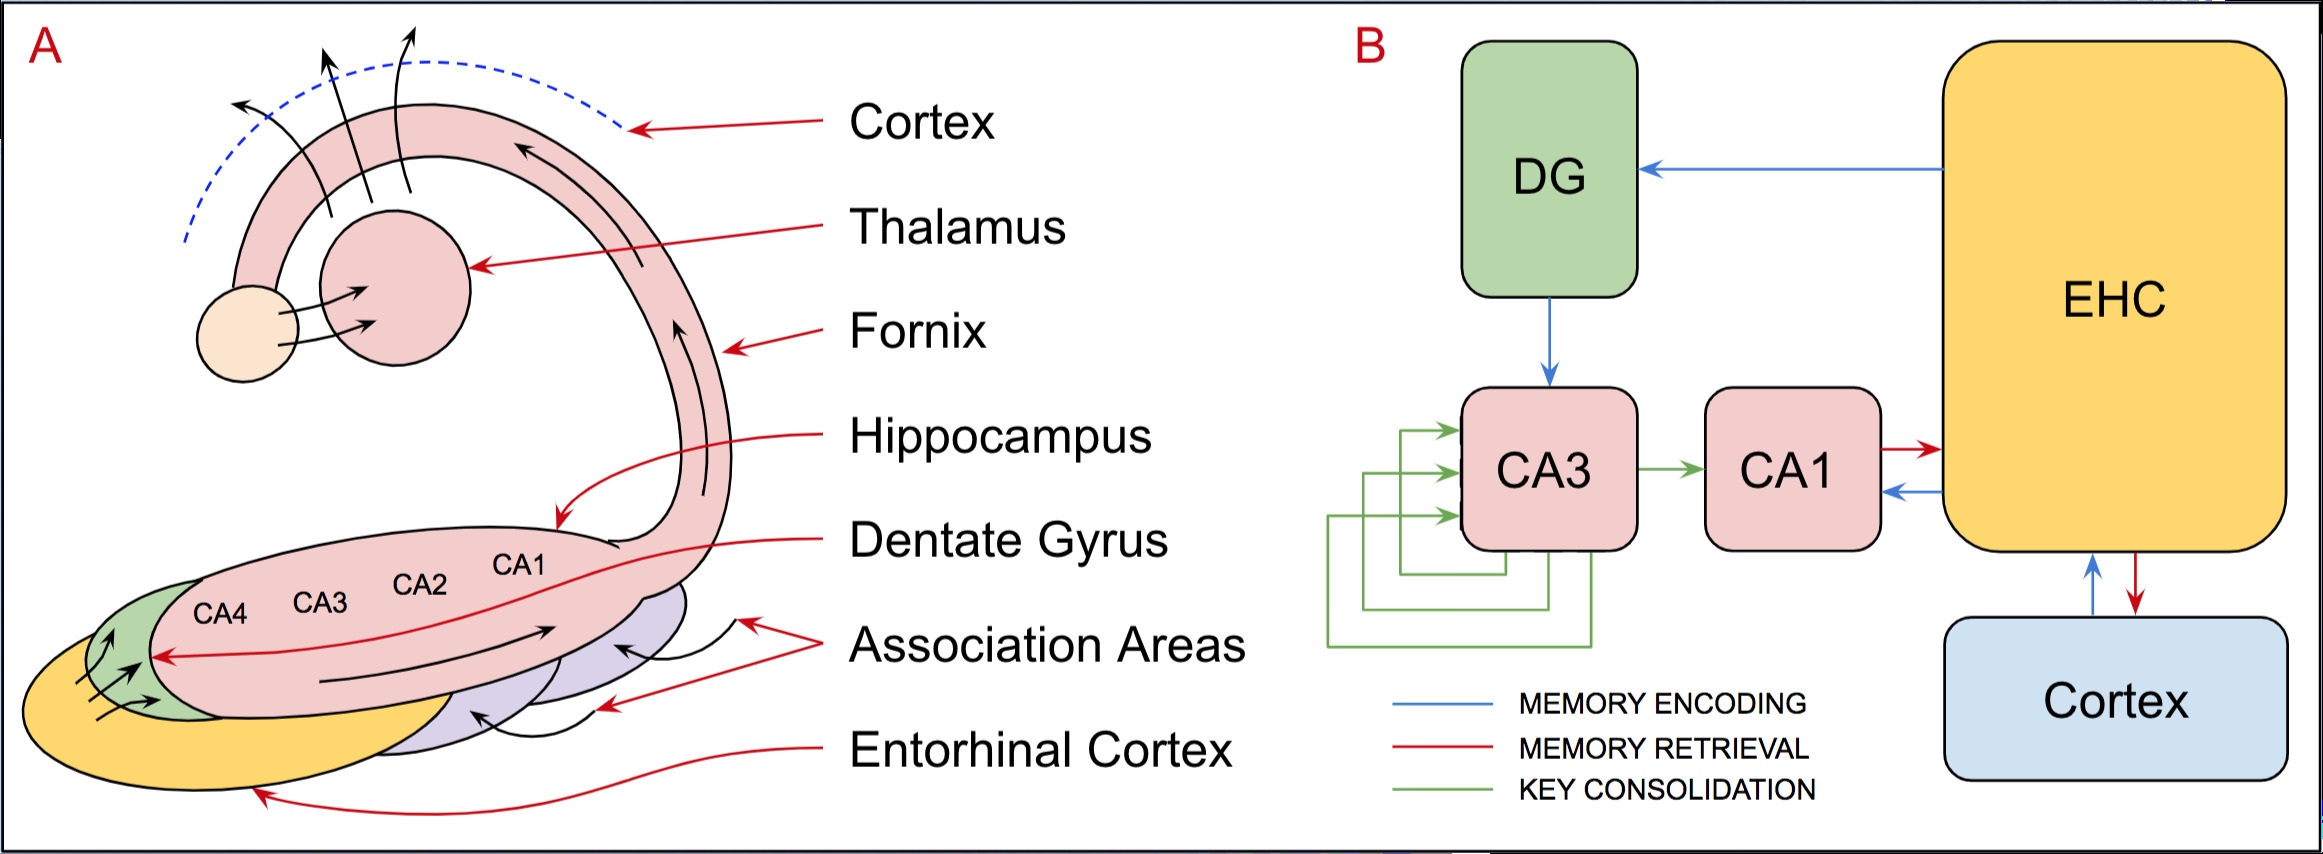
\includegraphics[width=4.0in]{./figures/Hippocampus_Anatomy_and_Physiology.png} %%% 2362 × 900 pixels @ 72 per inch
  \end{center}
%
  \caption{On the left you see a cartoon drawing of the hippocampus and related cortical and subcortical areas. The primary components include the entorhinal cortex or EHC, the dentate gyrus or DG and two hippocampal (out of four) nuclei referred to as CA3 and CA1. Figure~\ref{fig_broadman} provides additional anatomical detail regarding the connections between cortical regions and the perirhinal and parahippocampal areas adjacent to the hippocampus. The block diagram on the right summarizes the component circuits, along with their projections and reciprocal connections.}
%
  \label{fig_hippo}
%
\end{figure}

%%% %%%%%%%%%%%%%%%%%%%%%%%%%%%%%%%%%%%%%%%%%%%%%%%%%%%%%%%%%%%%%%%%%%%%%%%%%%%%

The name {\it{hippocampus}} like so many biological terms has obscure origins, generally in Latin or Greek and in this case the latter, relating to its shape that looked like a seahorse to some early anatomists. As shown in Figure~{\urlh{#fig_Hippocampus_Anatomy_and_Physiology}{\ref{fig_hippo}}} ({\colorred{A}}) it is primarily comprised of four subnuclei referred to as CA1, CA2, CA3 and CA4, the first two characters in each abbreviation recalling a previous Latin name, {\it{Cornu Ammanonis}} associated with a ram's horn, apparently preferred by even earlier anatomists. These nuclei are capped by the {\it{dentate gyrus}} (DG) at one end and the {\it{fornix}} at the other\footnote{%
%
  The hippocampus plays an important role in the transfer of information from short-term memory to long-term memory during encoding and retrieval stages. These stages need not occur successively, but are broadly divided in the neuronal mechanisms they require or even in the hippocampal areas they activate. According to Michael Gazzaniga, "encoding is the processing of incoming information that creates memory traces to be stored." There are two steps to encoding: acquisition and consolidation. During acquisition, stimuli are committed to short term memory. Consolidation is where the hippocampus along with other cortical structures stabilize an object within long term memory. ({\urlh{https://en.wikipedia.org/wiki/Hippocampal_memory_encoding_and_retrieval}{SOURCE}})}. 

The hippocampus consists of two nearly identical structures, one in each hemisphere, connected where the parallel tracts of the fornix come together at the midline of the brain. The hippocampus is tightly coupled with the {\it{entorhinal cortex}} (EHC) that plays an important role in memory, navigation and our perception of time. Information flows from the EHC to the hippocampus by one of two pathways: either through the DG to CA3 or via reciprocal connections to and from CA1. The EHC also has reciprocal connections to many cortical areas. Figure~{\urlh{#fig_Brodmann_Basal_Ganglia_Hippocampus}{\ref{fig_broadman}}} ({\colorred{A}}) provides additional anatomical detail. 

In the process of creating a new memory, the hippocampus receives input from multiple cortical areas relevant to current experience, consolidates this information in a condensed format that will enable subsequent retrieval and stores the resulting encoding in memory. In retrieving an existing memory, The EHC starts with cortical activity, typically from motor and sensory association areas, and uses this information to reconstruct a previous memory by activating cortical areas corresponding to the original memory. Before describing how we think such creative consolidation and subsequent reconstruction works, a word about why this process is beneficial might be in order.

Almost every stage of memory is fraught with opportunities to alter stored representations of prior experience. Reconstruction is a creative process in which we are more often than not forced to fill in some details that we might think we observed at the time but actually didn't. In the formation of new memories, consolidation can only make do with whatever information about the experience we have gleaned from observation and committed to short-term memory. If you don't rehearse what you've stored in short-term memory then it will quickly fade, losing detail and potentially introducing errors of omission and commission.

%%% You might purposely or unconsciously alter what you think you remember to conveniently leave the impression that you behaved different than you actually did. There are all kinds of reasons to alter your memories to suit your purposes just as there all sorts of reasons for lying to ourselves~\cite{Trivers2011}. Self-deception can offer interpersonal benefits that offset its costs in whatever currency you value most. There is evidence to suggest that people lie to convince themselves of the truth of their persuasive goal, and by doing so, are able to argue their case more persuasively to others~\cite{SmithetalJEP-17}. 

%%% This sort of imaginative reconstruction has called into question the accuracy of first-person accounts and expert witnesses. But it also explains our eminently useful commonsense application of believable counterfactual reasoning, e.g., if I hadn't had that second cup of coffee, I would have slept better last night~\cite{ParikhetalNEUROIMAGE-18,DeBrigardetalNEUROIMAGE-15}. And, considered in the context of avoiding dangerous situations, planning for contingencies, or imagining a world very different from the one in which we live, one that can inspire and motivate us to act to achieve such a future, it underscores the amazing strength, resilience and determination of the human mind.

The basic algorithm carried out by the hippocampus and entorhinal cortex working together is illustrated in Figure~{\urlh{#fig_Hippocampus_Anatomy_and_Physiology}{\ref{fig_hippo}}} ({\colorred{B}}). There are two basic processes that we consider here: encoding new memories and retrieving old memories. Encoding involves collecting information gleaned from diverse neural activity originating in multiple cortical regions and consolidating~\cite{MorrisetalNEURON-06} this information to construct a compact encoding that serves as a key or index that will enable subsequent stable \emdash{} meaning reliably consistent even in the presence of distracting information~\cite{EisenbergetalSCIENCE-03} \emdash{} retrieval and reconstruction\footnote{% 
%
   Memory consolidation is a category of processes that stabilize a memory trace after its initial acquisition. Consolidation is distinguished into two specific processes, synaptic consolidation, which is synonymous with late-phase long-term potentiation and occurs within the first few hours after learning, and systems consolidation, where hippocampus-dependent memories become independent of the hippocampus over a period of weeks to years. Recently, a third process has become the focus of research, reconsolidation, in which previously-consolidated memories can be made labile again through reactivation of the memory trace. ({\urlh{https://en.wikipedia.org/wiki/Memory_consolidation}{SOURCE}})}.

EHC receives input from all cortical regions in a condensed form and the axons of EHC pyramidal neurons project primarily to the DG but also to CA1. DG then projects to CA3 which plays a particularly important role in encoding and retrieving memories. CA3 is thought to behave as an autoassociative memory shown here as a recursive neural network. The crucial property of an autoassociative memory is that it is able to retrieve an item from memory using only a portion of the information associated with that item\footnote{%
% 
  {\it{Autoassociative memories}} are capable of retrieving a piece of data upon presentation of only partial information. {\it{Hopfield networks}} are recurrent artificial neural networks that have been shown to act as an autoassociative memory since they are capable of remembering data by observing a portion of that data. Hopfield networks can be trained with a variety of different learning methods including Hebbian learning which is often summarized as "neurons that fire together wire together". ({\urlh{https://en.wikipedia.org/wiki/Hopfield_network}{SOURCE}})}. 

%%% For example, this property allows us to retrieve information about a party that was held years ago just by catching a glimpse of a person on the street who happens to look like someone whom we first met at that party. You can think of your observation of the person from the party as a probe or key that enables you to access and unlock that earlier experience. Of course, you could have simply mistaken that person you saw on the street for the person you met at the party.

%%% Hippocampal indexing theory~\cite{TeylerandDiScennaBEHAVIORAL-NEUROSCIENCE-86} hypothesizes that when we have a conscious experience, different areas of the cortex are activated related to that experience such as activity in the auditory cortex resulting from our listening to a recording of Yo-Yo Ma playing Bach or activity in the visual cortex produced by a particularly vivid sunset we witnessing. When we remember the experience later, similar areas of the cortex are reactivated allowing us to re-experience the event.

The hippocampus serves as an index, storing different patterns of cortical activity and allowing us to retrieve our memories using only a fragment of what we can recall. The recurrent connections of CA3 are thought to enable this sort of creative reconstruction and play a role in both encoding and retrieving memories. CA3 then projects to CA1 and from there back to the EHC completing the loop and thereby providing recurrent activity involving a much larger circuit.

%%% %%%%%%%%%%%%%%%%%%%%%%%%%%%%%%%%%%%%%%%%%%%%%%%%%%%%%%%%%%%%%%%%%%%%%%%%%%%%

There are a couple of details that are worth pointing out here as they demonstrate both the strengths and weaknesses of human episodic memory. The first concerns the issue of retrieving a complete memory given a partial index and the second concerns how to retrieve a memory when that memory is similar to one or more other memories, at least in the sense that their respective indices are similar to one another. In the model described here, the first issue is handled by the autoassociative network.

%%% %%%%%%%%%%%%%%%%%%%%%%%%%%%%%%%%%%%%%%%%%%%%%%%%%%%%%%%%%%%%%%%%%%%%%%%%%%%%

%%% Figure~{\urlh{#fig_Hippocampus_Auto_Associative_Network}{\ref{fig_assoc}}}
\begin{figure}
%
  \begin{center}
%    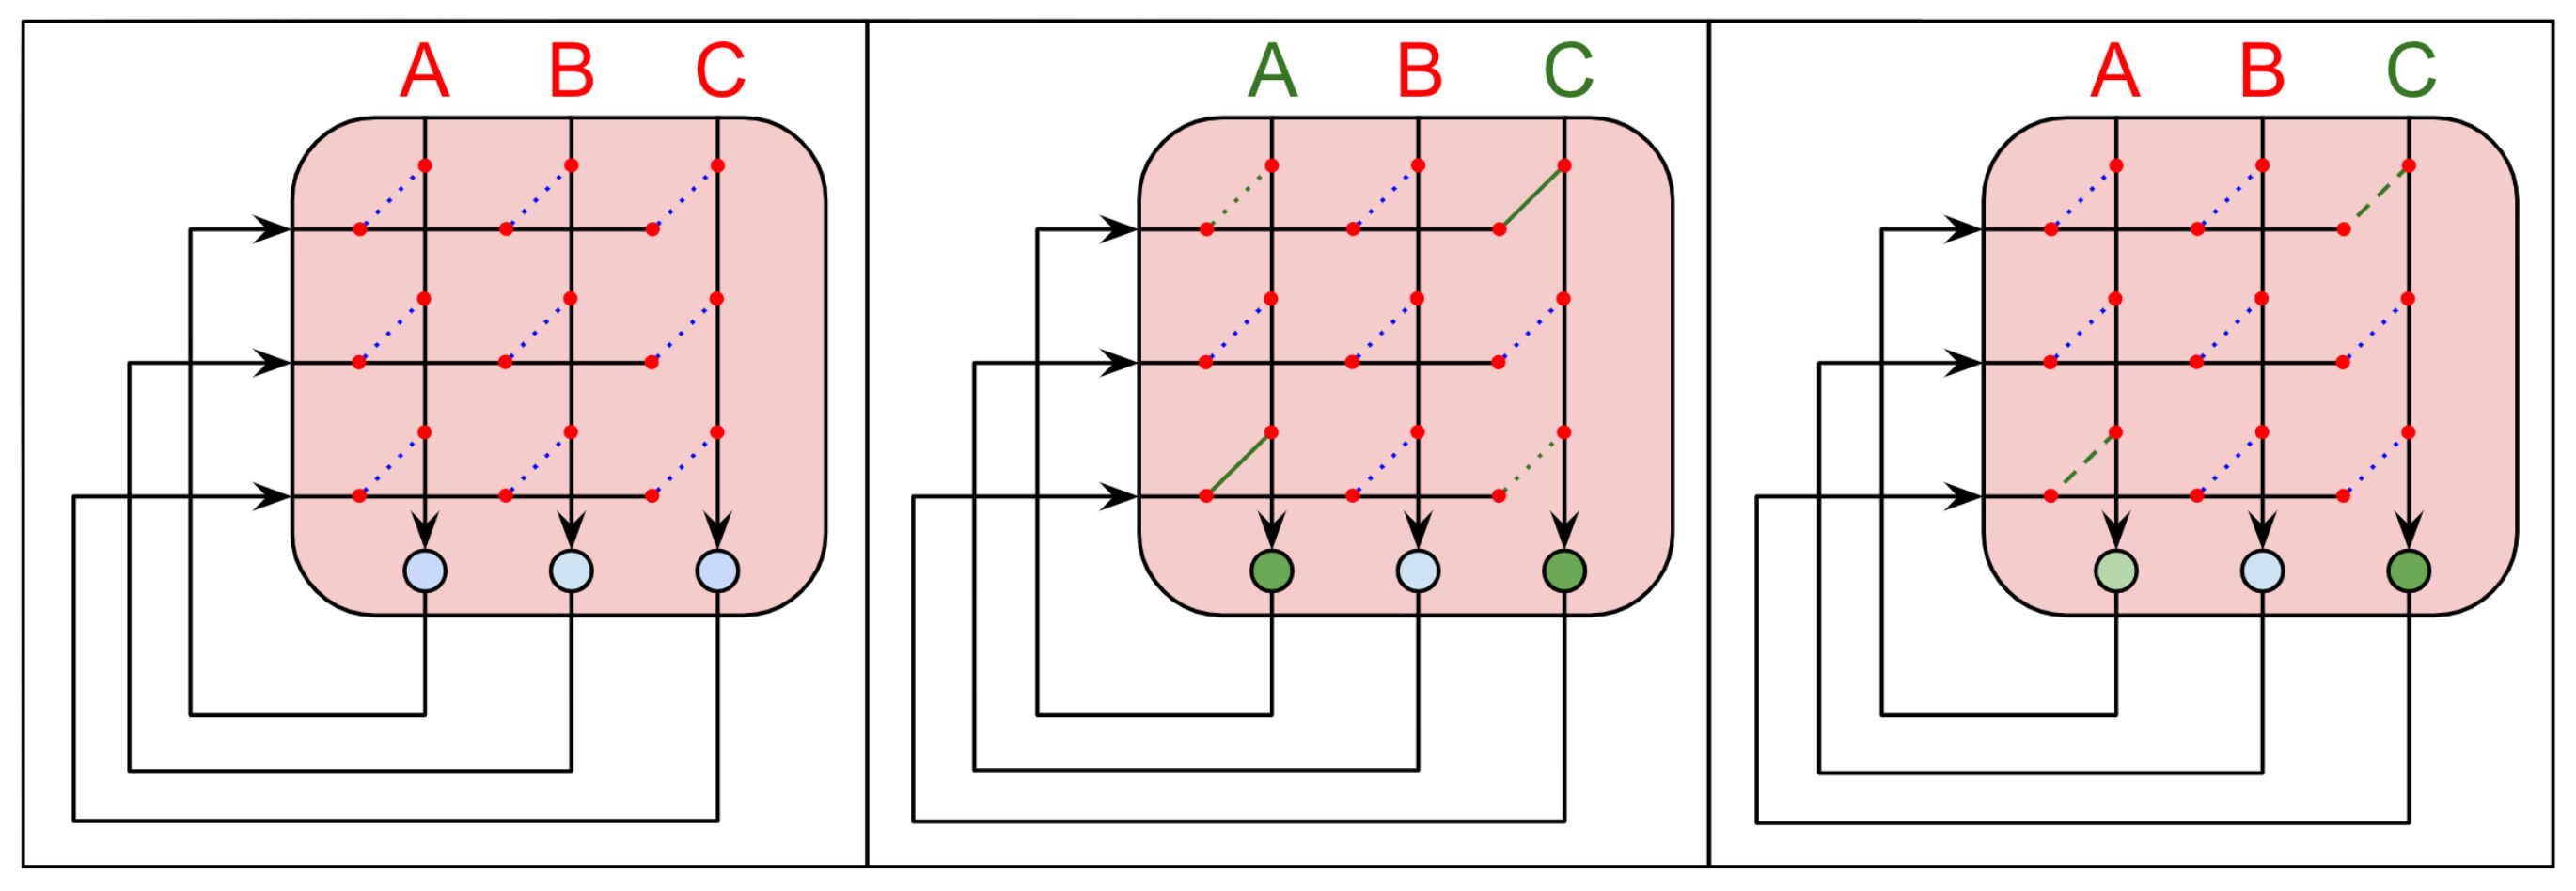
\includegraphics[width=7.5in]{./figures/Hippocampus_Auto_Associative_Network.png} %%% 2540 × 887 pixels
    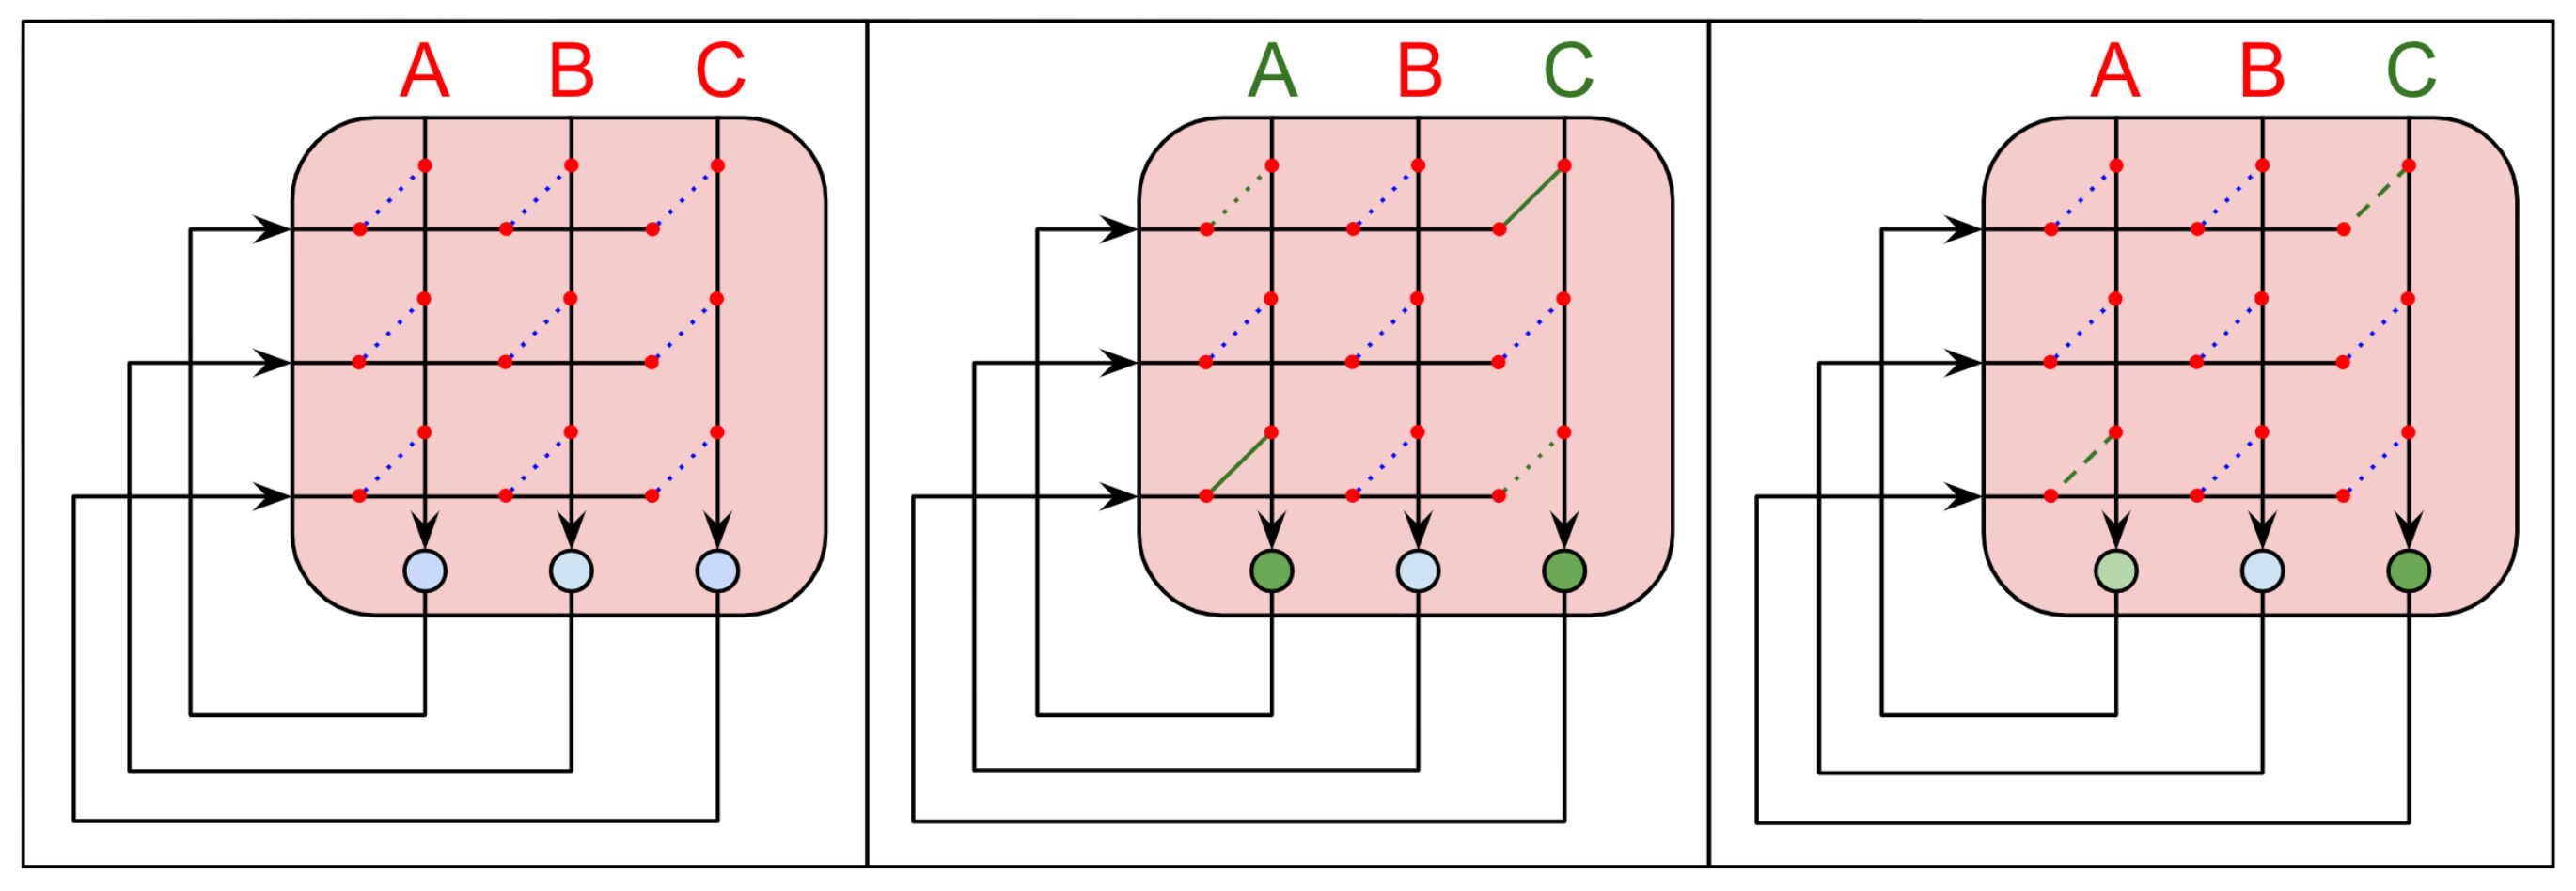
\includegraphics[width=3.25in]{./figures/Hippocampus_Auto_Associative_Network.png} %%% 2540 × 887 pixels
  \end{center}
%
  \caption{The three panels shown here represent the autoassociative network representing the function of CA3 in the hippocampus. Connection weights are shown as diagonal lines, e.g., the dotted blue lines shown in the network on the far left represent the connection weights prior to any training. The middle panel represents the network after encoding the stimulus pattern corresponding to the cortical activation of A and C, and the panel on the far right represents the network, when presented with a partial pattern consisting of just C, employing the recurrent connections of the autoassociator to complete the pattern for the original stimulus and using it to reconstruct the corresponding activation of A and C in the cortex.}
%
  \label{fig_assoc}
%
\end{figure}

%%% %%%%%%%%%%%%%%%%%%%%%%%%%%%%%%%%%%%%%%%%%%%%%%%%%%%%%%%%%%%%%%%%%%%%%%%%%%%%

The triptych shown in Figure~{\urlh{#fig_Hippocampus_Auto_Associative_Network}{\ref{fig_assoc}}} illustrates how the autoassociative network solves this problem. The panel on the far left is meant to indicate the autoassociative network and its initial state. In the middle panel, we assume the input from the dentate gyrus consist of the two sub patterns A and C and illustrates the reciprocal connections that would be strengthened were we to train the network with this composite pattern of activity. CA3 is responsible for encoding these memory specific patterns of activity for all of our memories.  The panel on the far right is intended to illustrate how given a partial pattern, in this case just one of the two representative patterns that comprise the composite pattern shown in the middle panel, is able to reconstruct the other representative pattern by using the trained autoassociative network to first identify and then strengthen the connections in the original composite.

The second detail concerns the possibility that the encodings for two memories are alike enough to be mistaken with one another. A full account of any of the theories explaining how the human brain solves this problem is beyond the scope of what we can go into here but one theory \emdash{} first articulated by David Marr~\cite{MarrandBrindleyPTRS_B-71,WillshawetalPTRS_B-15} \emdash{} posits that, since the dentate gyrus has a larger number of cells than the EHC, its forward projection will tend to produces an expansion recoding in the DG leading to an increase in the separation between the patterns in CA3. %%% Evidence from recordings in mice and computational modeling using artificial neural network and dynamical system models offer support for the theory~\cite{NeunuebelandKnierimNEURON-14}. 

%%% %%%%%%%%%%%%%%%%%%%%%%%%%%%%%%%%%%%%%%%%%%%%%%%%%%%%%%%%%%%%%%%%%%%%%%%%%%%%

%%% Memory consists of patterns of cortical activations which can be condensed and
%%% sent to the entorhinal cortex, undergo pattern separation and then bound together
%%% are indexed in the CA3 auto associator.  

%%% Then when a feature of the original stimulus is present it activates a subpopulation
%%% of the original neurons activated in the CA3 and the recurrent connections reactivate
%%% the remaining neurons making up the pattern,

To complete our account of memory retrieval, we look at how the path that started in the EHC loops back to complete a feedback loop that stabilizes the encoding of memories. So far we've seen how an experience represented by a pattern of activity in the cortex is compressed and represented in the entorhinal cortex which projects this pattern onto the cells in the dentate gyrus thereby increasing the separation between competing patterns the results of which are bound together to generate an index. This index is fed to CA3 where it is incorporated in an autoassociative recursive network so that subsequently when a feature of the original stimulus is present in our conscious experience it activates a subset of the original neurons activated in CA3 and the recurrent connections in the autoassociative network reactivate the remaining neurons completing the pattern that was incorporated when the experience was initially encoded in memory.
  
%%% The final step is to see how the reactivates the original stimulus. This is thought
%%% to be mediated by CA1. The entorhinal cortex not only projects to the dentate gyrus,
%%% it also projects to CA1.

%%% This means that when the neurons are activated in CA3, also activated in CA1 is
%%% another representation of the cortical path. Since these populations of neurons are
%%% activated at the same time, they undergo long-term potentiation and the connections
%%% between them are strengthened.

%%% The above account provides a clear unique role for every area in the system, except
%%% for area CA1 - what is the unique role of CA1? In the original CLS work,
%%% including McClelland and Goddard (1997), we theorized that CA1 is critical for
%%% developing a sparse, invertible mapping. This means that activity patterns produced
%%% by incoming cortical activity during encoding are capable of re-creating those same
%%% cortical activity patterns during retrieval without which, catastrophic interference
%%% would remain, regardless of how effective the pattern separation is within the CA3.

The remaining step involves explaining how the representation in CA3 reactivates the original stimulus. As shown in Figure~{\urlh{#fig_Hippocampus_Anatomy_and_Physiology}{\ref{fig_hippo}}} ({\colorred{B}}), the entorhinal cortex projects to CA1 in addition to the dentate gyrus. When neurons are projected forward to DG and activated in CA3 they are also activated in CA. Since they are activated at the same time, the connections between the neurons in CA3 and CA1 are strengthened by long-term potentiation\footnote{%
%
  In neuroscience, long-term potentiation (LTP) is a persistent strengthening of synapses based on recent patterns of activity. These are patterns of synaptic activity that produce a long-lasting increase in signal transmission between two neurons. The opposite of LTP is long-term depression, which produces a long-lasting decrease in synaptic strength. It is one of several phenomena underlying synaptic plasticity, the ability of chemical synapses to change their strength. As memories are thought to be encoded by modification of synaptic strength, LTP is widely considered one of the major cellular mechanisms that underlies learning and memory. ({\urlh{https://en.wikipedia.org/wiki/Long-term_potentiation}{SOURCE}})}.
%
The result is a stable, sparse, invertible mapping that allows the hippocampus to recreate the original cortical activity patterns during retrieval~\cite{OReillyetalCS-15,McClellandandGoddardHIPPOCAMPUS-97}. Reactivating the same combination of cortical areas as the original stimulus and causing us to reexperience the event as a memory. An additional process called {\it{reconsolidation}} is thought to allow previously-consolidated memories become labile again as a consequence of reactivation\footnote{%
%
  Memory reconsolidation is the process of previously consolidated memories being recalled and actively consolidated. It is a distinct process that serves to maintain, strengthen and modify memories that are already stored in the long-term memory. Once memories undergo the process of consolidation and become part of long-term memory, they are thought of as stable. However, the retrieval of a memory trace can cause another labile phase that then requires an active process to make the memory stable after retrieval is complete. It is believed that post-retrieval stabilization is different and distinct from consolidation, despite its overlap in function. ({\urlh{https://en.wikipedia.org/wiki/Memory_consolidation}{SOURCE}})}.
%
See {\urlh{box_patterns}{Box~\colorred{A}}} for detail on storing and retrieving memories in the hippocampus.

%%% %%%%%%%%%%%%%%%%%%%%%%%%%%%%%%%%%%%%%%%%%%%%%%%%%%%%%%%%%%%%%%%%%%%%%%%%%%%%
   
%%% This means that neurons in CA3 activate the neurons in CA1 corresponding to the
%%% correct cortical areas. These then project back to the entorhinal cortex which
%%% has reciprocal connections to many areas of the cortex. Reactivating the same
%%% combination of cortical areas as the input and causing us to reexperience the
%%% event as a memory.

%%% %%%%%%%%%%%%%%%%%%%%%%%%%%%%%%% END HIPPOCAMPAL COMPLEX %%%%%%%%%%%%%%%%%%%%%%%%
